% The methods for implementation of a behavioral, discrete-time PLL simulator and for the PLL loop filter automation and optimization will be covered here.

% \hl{Talk about how simulator is implemented:}
% \hl{Discrete simulation models of phase noise, dco etc}
% \hl{Filter optimization}
% \hl{-phase noise and lock time estimate in frequency domain}


\section{ADPLL Design Automation}
Design automation for ADPLL loop filter is implemented with a strategy that utilizes a continuous time-approximation based model of the PLL to generate a pseudo-optimum loop filter design, and then performs discrete time conversion and digitization of the design. Second order optimization is then applied to the discretized and digitized filter implementation, to minimize effects of quantization error and filter design error due to finite word effects. A discrete-time, behavioral PLL simulator is then used to verify the filter design for proper lock-time, phase noise and stability.

The design automation approach utilizes a fixed form of a loop filter as a prototype for all loop filter designs. 

\subsection{Loop filter}
\subsection{Design sequence}

\section{Behavioral ADPLL simulation}
To fully capture the effects of a discrete time PLL with digital quantization effects, the implementation a behavioral, discrete event PLL simulator is described in the following. The simulator utilizes behavioral models to describe the individual components which comprise the PLL. These components are (1) a clock reference, (2) a TDC, (3) a loop filter, (4) a DCO, and (5) a divider. These behavioral models fully encapsulate effects of time-quantization and digitization. The simulator operates by iterating in fixed time steps of $\Delta t$=1/\texttt{fs}, where each node in the PLL is updated based upon the previous node values in a manner that is defined by each PLL component behavioral model. Each behavioral model is represented programmatically utilizing classes. In simulation, each component instance is represented by a object instance of the respective model class, constructed with any initial parameters (such as division ratio) that describe the component.
\begin{figure}[htb!]
	\center\fontfamily{\sfdefault}\selectfont
% XCircuit output "simulator.tex" for LaTeX input from simulator.ps
\def\putbox#1#2#3#4{\makebox[0.00000in][l]{\makebox[#1][l]{}\raisebox{\baselineskip}[0.00000in][0.00000in]{\raisebox{#2}[0.00000in][0.00000in]{\scalebox{#3}{#4}}}}}
\def\rightbox#1{\makebox[0.00000in][r]{#1}}
\def\centbox#1{\makebox[0.00000in]{#1}}
\def\topbox#1{\raisebox{-0.60\baselineskip}[0.00000in][0.00000in]{#1}}
\def\midbox#1{\raisebox{-0.20\baselineskip}[0.00000in][0.00000in]{#1}}
   \scalebox{1}{
   \normalsize
   \parbox{6.30936in}{
   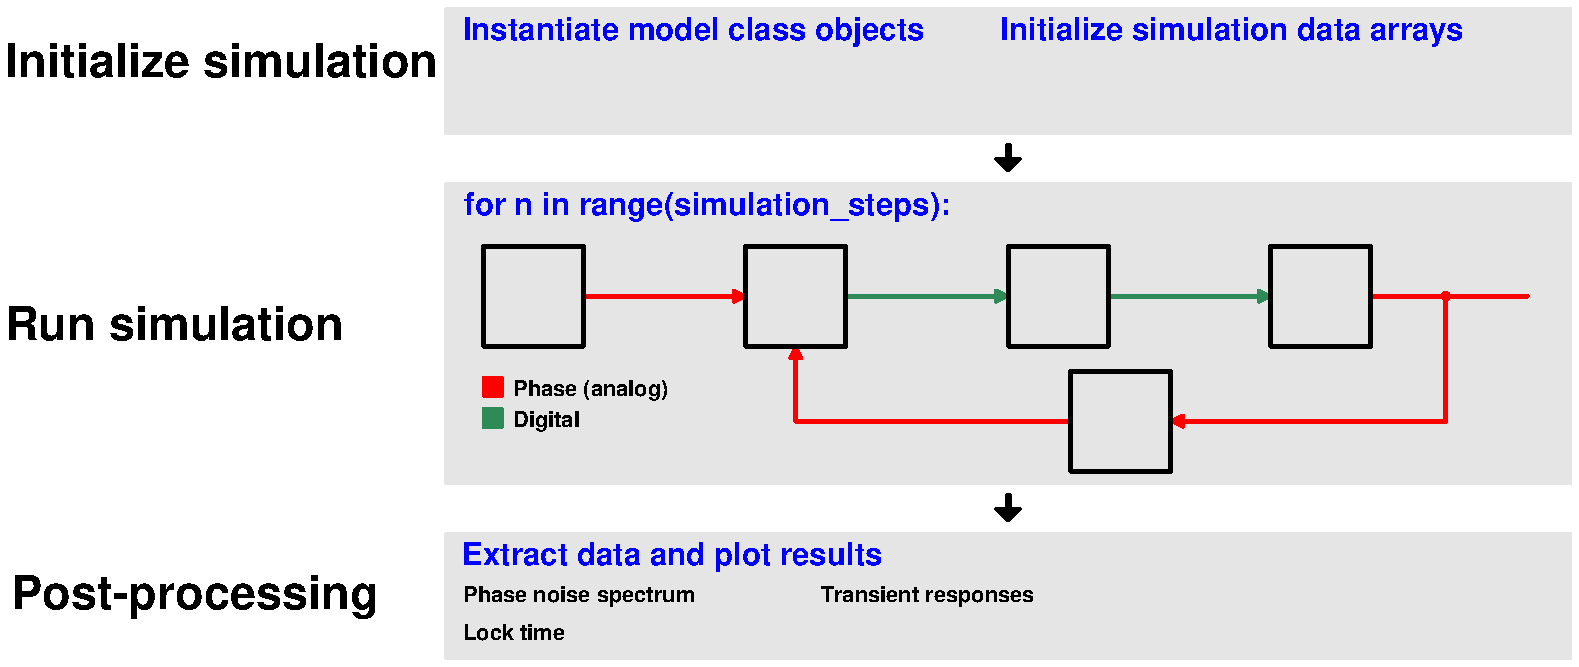
\includegraphics[scale=0.60000]{./figs/simulator.pdf}\\
   % translate x=1040 y=384 scale 0.38
   \putbox{3.08400in}{1.45800in}{0.84}{\texttt{tdc}}%
   \putbox{4.38600in}{0.96000in}{0.84}{\texttt{div}}%
   \putbox{4.17000in}{1.45800in}{0.84}{\texttt{lf}}%
   \putbox{5.18400in}{1.45800in}{0.84}{\texttt{dco}}%
   \putbox{2.03400in}{1.45800in}{0.84}{\texttt{clk}}%
   \putbox{3.48600in}{1.03200in}{0.84}{\texttt{div\_sig[n]}}%
   \putbox{2.38200in}{1.56000in}{0.84}{\texttt{clk\_sig[n]}}%
   \putbox{3.43200in}{1.54800in}{0.84}{\texttt{tdc\_sig[n]}}%
   \putbox{4.48200in}{1.54800in}{0.84}{\texttt{lf\_sig[n]}}%
   \putbox{5.53200in}{1.54800in}{0.84}{\texttt{dco\_sig[n]}}%
   \putbox{4.00800in}{2.35800in}{0.84}{\texttt{clk\_sig[n]}}%
   \putbox{4.00800in}{2.20800in}{0.84}{\texttt{tdc\_sig[n]}}%
   \putbox{4.71000in}{2.35800in}{0.84}{\texttt{lf\_sig[n]}}%
   \putbox{4.71000in}{2.20800in}{0.84}{\texttt{dco\_sig[n]}}%
   \putbox{5.38200in}{2.35800in}{0.84}{\texttt{div\_sig[n]}}%
   \putbox{1.86000in}{2.35800in}{0.84}{\texttt{clk}}%
   \putbox{1.86000in}{2.20800in}{0.84}{\texttt{tdc}}%
   \putbox{2.40600in}{2.35800in}{0.84}{\texttt{lf}}%
   \putbox{2.40600in}{2.20800in}{0.84}{\texttt{dco}}%
   \putbox{2.95800in}{2.35800in}{0.84}{\texttt{div}}%
   \putbox{1.88400in}{0.83400in}{0.84}{t$_{sim}$ = \texttt{n}$\Delta$t}%
   \putbox{2.73600in}{3.09600in}{0.72}{\texttt{fref}}%
   \putbox{2.55600in}{2.99400in}{0.72}{\texttt{div\_n}}%
   \putbox{2.49600in}{2.89800in}{0.72}{\texttt{tdc\_steps}}%
   \putbox{3.60600in}{3.09600in}{0.72}{\texttt{kdco}}%
   \putbox{4.20600in}{2.99400in}{0.72}{\texttt{dco\_f0}}%
   \putbox{4.20600in}{2.89800in}{0.72}{\texttt{dco\_pn}}%
   \putbox{5.64600in}{3.09600in}{0.72}{\texttt{init\_f\_error}}%
   \putbox{5.18400in}{2.99400in}{0.72}{\texttt{lf\_params}}%
   \putbox{5.44800in}{2.89800in}{0.72}{\texttt{sim\_steps}}%
   } % close 'parbox'
   } % close 'scalebox'
   \vspace{-\baselineskip} % this is not necessary, but looks better
\fontfamily{\rmdefault}\selectfont

	\caption{Simulation process.}
	\label{fig:simulator}
\end{figure}
\FloatBarrier
The discrete event simulator is given in the following pseudocode, with component model objects \{\texttt{clk, tdc, lf, dco, div}\}, and simulation data arrays \{\texttt{clk\_sig, tdc\_sig, lf\_sig, dco\_sig, div\_sig}\}. Each model object is updated at each simulation step utilizing the class method \texttt{update}, passing any relevant simulation data as arguments to the method.

\begin{lstlisting}[language={Python}, caption={PLL simulation loop Python pseudocode}, label={sim_code}]
for n in range(simulation_steps):
    clk_sig[n] = clk.update()
    tdc_sig[n] = tdc.update(clk_sig[n-1], div_sig[n-1]))
    lf_sig[n]  = lf.update(tdc_sig[n-1], clk_sig[n-1]) #loop filter
    osc_sig[n] = dco.update(lf_sig[n-1])
    div_sig[n] = div.update(osc_sig[n-1], div_n)
    \end{lstlisting}
After the simulation loop reaches completion, the results stored in the simulation data arrays can be post-processed to extract phase noise data, transient behavior and lock time. The following sections will discuss in more detail the implemented behavioral model classes and post-processing.

\subsection{Clock behavioral model}
An ideal behavioral clock model is utilized. The model is instantiated with the clock frequency \texttt{f} and the simulator time step \texttt{dt}. The model incrementing its phase every simulation step by a fixed amount $\Delta \Phi$ = $2\pi$\texttt{f}$\cdot$\texttt{dt}. The model outputs an analog phase signal.

\begin{lstlisting}[language={Python}, caption={Ideal clock behavioral model.}, label={clk_code}]
class Clock:
	def __init__(self, f, dt):
		self.f = f 			# clock frequency
		self.dt = dt 		# simulation time step
		self.phase = 0.0	# clock phase state variable

	def update(self):
		self.phase += 2*pi*self.f*self.dt 	# increment phase
		return self.phase
    \end{lstlisting}

\subsection{TDC behavioral model}
The TDC behavioral model takes two analog inputs \texttt{x} and \texttt{y} that are in units of phase, and outputs a digital word that quantifies the phase separation of the signals. The model is instantiated with a resolution parameter \texttt{tdc\_steps}, which defines the number of phase steps per cycle of the reference input \texttt{x} the TDC can resolve. The method \texttt{round} quantizes an floating point argument to the nearest integer.

\begin{lstlisting}[language={Python}, caption={TDC behavioral model.}, label={tdc_code}]
class TDC:
	def __init__(self, tdc_steps):
		self.tdc_steps = tdc_steps

	def update(x, y):
		ph_error = wrap(x-y) 	# wraps phase to be within [0, 2*pi]
		return round(self.tdc_steps*(ph_error/(2*pi)))
\end{lstlisting}
\subsection{Loop filter behavioral model}
The loop filter model implements a discrete-time filter via difference equation that operates on input \texttt{x}. The equivalent of one pole and two zeros are modelled, described using the filter coefficients $\{a_1, a_2; b_0, b_1\}$:
\begin{equation}
\text{H}_{LF}(z) = \frac{b_0 + b_1z^{-1}}{a_0 + a_1z^{-1} + a_2z^{-2}}
\end{equation}
\begin{equation}
\text{y}[n] = -a_1 \text{y}[n-1]-a_2 \text{y}[n-2] + b_0\text{x}[n] + b_1\text{x}[n-1]
\end{equation}
Pseudocode for implementation of the model class is as follows. Data is to be represented with fixed point format, with number of fractional bits \texttt{frac\_bits} and number of integer bits \texttt{int\_bits}. The method \texttt{fixed\_point} rounds floating point values to be equivalent to the nearest representation in the desired fixed point format. The filter coefficients are assumed to be pre-converted to the desired fixed-point equivalent values, and input \texttt{x} is assumed to be integer-valued.
\begin{lstlisting}[language={Python}, caption={Loop filter behavioral model.}, label={lf_code}]
class LoopFilter:
	def __init__(self, a1, a2, b0, b1, int_bits, frac_bits):
		self.a1 = a1;	self.a2 = a2
		self.b0 = b0;	self.b1 = b1
		self.xprev1 = 0;	
		self.yprev1 = 0; self.yprev2 = 0
		self.int_bits=int_bits;	self.frac_bits=frac_bits

	def update(x):
		ynew = -self.a1*self.yprev1 - self.a2*self.yprev2 \\
			   + self.b0*x + self.b1*self.xprev1	# difference equation
		self.yprev2 = self.yprev1	
		self.yprev1 = fixed_point(ynew, self.int_bits, self.frac_bits)
		self.xprev1 = x
		return round(self.yprev1)	# convert to integer
\end{lstlisting}

\subsection{DCO behavioral model}
The DCO is modeled similar to the clock model, with the inclusion of a digital input \texttt{otw} for tuning the frequency. Nominal oscillator frequency is given by \texttt{f0}, and the DCO gain in Hz/LSB of \texttt{otw} is \texttt{kdco}. Additionally, oscillator phase noise modeling is included utilizing additive random phase walk (see section \ref{dco_noise}). Random walk is implemented by stochastically adding or subtracting a fixed magnitude random walk phase increment $\texttt{krw}$ to the oscillator phase every simulation step. The sign of \texttt{krw} is randomly chosen with equal probability for positive and negative, implemented with the method \texttt{choice}.

\begin{lstlisting}[language={Python}, caption={DCO behavioral model.}, label={dco_code}]
class DCO:
	def __init__(self, f0, kdco, krw):
		self.f0 = f0		# nominal frequency
		self.kdco = kdco 	# DCO gain
		self.krw			# random phase walk gain
		self.phase = 0		# phase state variable

	def update(otw):
		self.phase += 2*pi*(f0 + otw*kdco) + krw*choice([-1,1])
		return self.phase
   \end{lstlisting}

\subsection{Divider behavioral model}
The divider model is definied with the divider modulus \texttt{div\_n} and only performs a simple division of input phase. 
\begin{lstlisting}[language={Python}, caption={Divider behavioral model.}, label={div_code}]
class Divider:
	def update(x, div_n):
		return x/div_n
\end{lstlisting}

\subsection{Post processing: lock time detection}
Lock time detection of the PLL start-up transient can be determined from the simulation data conditioned on a tolerance band for acceptable frequency error \texttt{lock\_f\_tol} is provided to the simulator by the user. Since the desired frequency of the PLL \texttt{fosc = div\_n*fref}, nominal oscillator frequency \texttt{dco\_f0} and simulation conditions of the PLL are known by the simulator, the ideal value of the loop filter at lock, \texttt{lf\_lock\_ideal} can be computed directly. Given the DCO gain value in the simulation \texttt{kdco}, the value of \texttt{lf\_lock\_ideal = round((fosc - dco\_f0)/kdco)}. Lock is then detected at the first simulation step for which the current and all later time steps meet the following criteria for the loop filter signal \texttt{lf\_sig} (i.e. frequency of oscillator is within the frequency tolerance band):
\begin{equation}
\text{\texttt{abs(lf\_sig[n] - lf\_lock\_ideal)*kdco < lock\_f\_tol}}
\end{equation}
This measurement is predicated on the simulation being fully complete at the time of measurement. Lock time is computed by multiplying the simulation index of lock with the simulation time step, 1/\texttt{fs}.

\subsection{Post processing: phase noise power spectrum estimate}
The simulation data can be used to make an estimate of the single side band phase noise power spectrum $\mathcal{L}(\Delta f)$ of the PLL (normalized to the carrier power). First, the phase error signal of the simulated PLL must be computed, \texttt{phase\_error = div\_n*clk\_sig - osc\_sig}. The phase error signal includes the phase noise signal in addition to any transient phase error components of the PLL. If the simulated PLL is in lock, the phase error can be is dominated by phase noise components, as the transient components become negligible. If \texttt{phase\_error} is reduced to the simulation signal span after the detection of lock, with a span in samples of \texttt{n\_steps}, the power spectral density of the phase noise normalized to the carrier tone, utilizing the fast Fourier transform (FFT) is:
\begin{equation}
	\text{\texttt{psd}} = \left|\frac{1}{\text{\texttt{n\_steps}}}\cdot\mathcal{FFT}\{\text{\texttt{div\_n*clk\_sig - osc\_sig}}\}\right|^2
\end{equation}
Provided the simulation sampling rate \texttt{fs}, the indices [0, \texttt{n\_steps}/2-1] of the FFT and consequently \texttt{psd} correspond to frequencies [0, \texttt{fbin}$\cdot$(\texttt{n\_steps}/2-1)], where \texttt{fbin} = \texttt{fs}/\texttt{n\_steps}. Slicing the power spectrum data \texttt{psd} with indices [1, \texttt{fbin}$\cdot$(\texttt{n\_steps}/2-1)] will yield the single side band spectrum of the oscillator, with the corresponding offset frequency of each index \texttt{k} being $\Delta f$\texttt{k*fbin}. Thus:
\begin{equation}
	\mathcal{L}(\Delta f) = \text{\texttt{psd[round(}}\Delta f\text{\texttt{/fbin)]}}
\end{equation}

\subsection{Monte-Carlo sampling}
The simulation code implemented uses a Python dictionary containing the simulation parameters and the corresponsing parameters for which the simulation engine should simulate the PLL for. This format makes the introduction of Monte-Carlo sampling into the simulator straightforward. This can be implementing utilizing a dictionary with the nominal simulation configuration, and then a second dictionary to define the parameters to be varied along with the corresponding parameter variance. Given a sample size of N for the Monte-Carlo simulation, a loop is implemented which creates a new simulation configuration dictionary each loop iteration with stochastically sampled values from a normal distribution based on the provided nominal configuration and variance dictionaries. That unique configuration dictionary instance is used to spawn a PLL simulation, and is stored. After N iterations, N sets of data are created with varied parameters.

\section{Loop filter optimization}
The loop filter optimization engine implemented utilizes constrained optimization to minimize total phase noise of the PLL subject to lock time constraints. The optimizer is limited to optimizing for a loop filter in the form of \ref{eq:loop_filter_def}, having parameters $K_i$, $\omega_p$, $\omega_z$. Following the theory of section \ref{adpll_model}, the PLL will have open loop and normalized closed loop transfer functions $\mathrm{L}(s)$ and $\mathrm{\hat{T}}(s)$ in \ref{eq:loop_gain_def} and \ref{eq:norm_cl_def} respectively.  Computationally fast methods utilizing the continuous closed-loop PLL approximation $\mathrm{\hat{T}}(s)$ to estimate PLL settling time and phase noise are implemented as cost functions for the optimizer.

	\begin{equation}\label{eq:loop_filter_def}
	\mathrm{H}_{LF}(s) = \frac{K_i}{s}\frac{(\frac{s}{\omega_z}+1)}{(\frac{s}{\omega_p}+1)}
	\end{equation}
	\begin{equation}\label{eq:loop_gain_def}
	\mathrm{L}(s) = \frac{K}{s^2}\frac{(\frac{s}{\omega_z}+1)}{(\frac{s}{\omega_p}+1)}
	\end{equation}
	\begin{equation}\label{eq:norm_cl_def}
	\mathrm{\hat{T}}(s) = \frac{\mathrm{L}(s)}{1+\mathrm{L}(s)} = \frac{K}{s^2}\frac{(\frac{s}{\omega_z}+1)}{(\frac{s}{\omega_p}+1)}
	\end{equation}

Filter optimization follows the following sequency:
\begin{enumerate}
	\setlength\itemsep{-0.8em}
	\item Minimize integrated phase noise with $\mathrm{\hat{T}}(s)$ definition of closed loop behavior. Yields optimal $\{K, \omega_p, \omega_z\}$.
	\item Translate optimal parameters to prototype loop filter parameters, perform continuous to discrete time filter conversion.
	\item Optimize fixed point resolution of digital loop filter implementation for finite word effects.
\end{enumerate}

The following sections detail the optimizer methods implemented.

\subsection{Fast estimation of PLL settling time}
	Based on the continuous model approximation of ADPLL dynamics, the PLL closed loop phase transfer function $\mathrm{\hat{T}}(s)$ is defined as a rational function of two polynomial functions of s, with P poles and Z zeros. Such a transfer function is computationally represented with arrays A and B, containing the denominator and numerator polynomial coefficients.
	\begin{equation}\label{eq:pll_cl_tf}
	\mathrm{\hat{T}}(s) = \frac{\sum_{j=0}^Z b_js^j}{\sum_{k=0}^P a_ns^n}
	\end{equation}
	An estimate of the step response settling time of $\mathrm{T}(s)$ can by utilizing its representation in state space. This is given in \ref{eq:ss_rep}, with input vector $\mathrm{U}(s)$, state vector $\mathbf{X}(s)$, and output $Y(s)$. The state-space representation from a s-domain transfer function can be quickly solved computationally with available signal processing packages such as \texttt{scipy.signal} given the coefficent arrays A and B.
	% https://lpsa.swarthmore.edu/Representations/SysRepTransformations/TF2SS.html
	\begin{align} \label{eq:ss_rep}
		s\mathbf{X}(s) &= \mathbf{AX}(s) +\mathbf{B}\mathrm{U}(s)\\
		Y(s) &= \mathbf{CX}(s) +\mathbf{D}\mathrm{U}(s)
	\end{align}
	The set of k eigenvalues $\{\lambda_1, ... , \lambda_{N}\}$ corresponding to poles for the system are found as the roots of \ref{eq:ss_eigenvals} \cite{brockett_1965}.% The associated eigenvectors are found with \ref{eq:ss_eigenvecs}.
	\begin{align}
		|\mathbf{A} - \lambda \mathbf{I}| = 0\label{eq:ss_eigenvals}%\\
		%\mathbf{A} \mathbf{v}_k = \lambda_k\mathbf{v}_k \label{eq:ss_eigenvecs}
	\end{align}
	Imposing the constraint of number of poles P $>$ number of zeros Z, the system $\mathrm{T}(s)$ may be represented via partial fraction decomposition using the poles from the eigenvalues of state matrix $\mathbf{A}$ $\{\lambda_1, ... , \lambda_{N}\}$:
	\begin{equation}
		T(s) = \sum_{k=1}^{P} \frac{c_k}{s-\lambda_k}
	\end{equation}
	Inverse Laplace transformation shows the step response of the system will be a sum of exponentials:
	\begin{equation}
		y(t) = c_1e^{\lambda_1t} + ... + c_ke^{\lambda_kt}%, \hspace{1em} \mathbf{y(t)} = [ y(t) \hspace{0.5em}y^{'}(t)\hspace{0.5em} ...\hspace{0.5em} y^{(k)}(t)]^T
	\end{equation}

	% The state transition matrix $\mathbf{\Phi}_{\mathrm{T}}$ corresponding to the system $\mathrm{T}(s)$ is:
	% \begin{equation}
		% \mathbf{\Phi}_\mathrm{T} = (s\mathbf{I}-A)^{-1}
	% \end{equation}

	The dynamics of the step response are governed by the exponential components of y(t). If  $\{\lambda_1, ... , \lambda_N\} \in \mathds{C}$ where $\lambda_k=1/\tau_k+j\omega_K$, the real portion of each $\lambda_k$ will describe the transient behavior of each exponential, having time constant $\tau_k$. The long term settling of y(t) will be dominated by the exponential with the largest $\tau_k$, i.e. the dominant pole of the system. This estimate of settling time uses the dominant pole $\tau_k$ as a heuristic estimate for overall time constant of the system, $\tau$. Finally, settling time $t_s$ can be considered as the time interval required for the signal to drop within a tolerance band $\pm \delta_{tol} \textnormal{y}(\infty)$ about the final value $\textnormal{y}(\infty)$. Thus:
	\begin{equation}
		t_s = \tau\ln(\delta_{tol}) = \frac{\ln(\delta_{tol})}{\min(|\Re(\{\lambda_1, ... , \lambda_k\})|)}
	\end{equation}
	This settling time estimate is computationally fast, as it requires only (a) computation of state matrix $\mathbf{A}$, (b) computation of the eigenvalues of $\mathbf{A}$, and (c) computation of settling time from the eigenvalue with minimum real component.

\subsection{Estimation of PLL phase noise}
	\hl{It is assumed here that [DISCUSSION EXPLAINS WHY...]} the dominant output-referred phase noise contributions of the PLL are due to the DCO thermal noise and TDC quantization. If $S_{TDC}$ and $S_{DCO}$ are the PLL output-referred noise PSD respectively for the TDC and DCO noise sources from section \ref{pn_theory}, the total PLL output noise PSD $S_{\Sigma}(f)$ is estimated as \ref{eq:tot_pn_est}. N is the PLL divider modulus.
	\begin{align}\label{eq:tot_pn_est}
		S_{\Sigma}(f) &= S_{\Phi n_{TDC,out}}(f) + S_{\Phi n_{DCO,out}}(f)\\
		 &= \frac{1}{12f_{ref}}\left|2\pi\frac{\mathrm{N}}{\mathrm{M}}\hat{\mathrm{T}}(f)\right|^2 + \frac{S_{0\Phi n_{DCO}}}{f^2}\left|1-\hat{\mathrm{T}}(f)\right|^2
	\end{align}

	Given a bandwidth of interest $\Delta f$ (i.e. baseband bandwidth for radio applications), the total integrated phase noise power is:
	\begin{equation}
		P_{\phi noise} = 2\int_0^{\Delta f} S_{\Sigma}(f)df
	\end{equation}
	This can be computation solved for a grid of K values in the interval $\Delta f$, where each point represents a frequency bin $f_{bin}$ = $\Delta f$/K. Therefore this estimate is implemented as such:
	\begin{equation}
		\hat{P}_{\phi noise} = 2\sum_{k=0}^{K-1} S_{\Sigma}(kf_{bin})f_{bin}
	\end{equation}

\subsection{Loop filter optimization algorithm}
	The optimization algorithm in use is predicated on a fixed form for the filter being design, as in \ref{eq:loop_filter_def}, and consequenctly known and fixed open and closed loop transfer function forms. The prototype loop filter design in this work a contains a tunable pole $\omega_p$, a tunable zero $\omega_z$ and a gain parameter $K$. To allow the phase noise minimization and the constraint on maximum lock time to both have an impact in the optimization, the optimization is implemented with two nested levels. There is there is a lower level optimizer which will minimize phase noise given a fixed target for settling time. The higher level optimizer applies a constrained search for settling time, utilizing the lower level optimizer, that results in minimum phase noise. 

	\textbf{Level A - Minimize phase noise for fixed settling time.}\label{lf_opt}
	\begin{itemize}
		\setlength\itemsep{-0.8em}
		\item Minimize phase noise while maintaining fixed settling time = $t_s$.
		\item \textbf{Solution:} use two steps per interation until satisfactorily converged:
		\begin{enumerate}
			\setlength\itemsep{-0.8em}
			\item Minimize phase noise using pole/zeros locations (gradient descent).
			\item Tune K such that settling time = $t_s$ (golden section search).
		\end{enumerate}

	\end{itemize}
	\textbf{Level B - Optimize settling time given constraints.}
	\begin{itemize}
		\setlength\itemsep{-0.8em}
		\item Use golden section search to find optimal constrained settling time that has minimal phase noise using method from level A as cost function.
	\end{itemize} 

\subsection{Loop filter optimization - finite word effects}
Once a filter design has been optimized in the continuous domain following section \ref{lf_opt}, second order optimization is carried out to ensure the digitized, discrete implementation performs as expected in the presence of finite word effects. The optimized digital implementation provided here utilized fixed-point words for equal resolution throughout the datapath. The implemented second order optimization considers both the effect of loop filter quantization noise and transfer function error.

\textbf{Loop filter quantization noise optimization}

